\chapter{Sistemi lineari}
\lecture{4}{25 Nov. 12:11}{Richiami}
\section{Relazioni di equivalenza}

Una relazione si dice di equivalenza se gode di tutte e tre le
seguenti proprietà:

\begin{itemize}
  \item{\makebox[4cm]{Proprietà Riflessiva\hfill}
    \makebox[4cm]{$\forall a\in S\phantom{.}$\hfill} $a\sim a$}
  \item{\makebox[4cm]{Proprietà Simmetrica\hfill}
    \makebox[4cm]{$\forall a\sim b\phantom{.}$\hfill} $b\sim a$}
  \item{\makebox[4cm]{Proprietà Transitiva\hfill}
      \makebox[4cm]{$\forall a\sim b, \forall b\sim
    c\phantom{.}$\hfill} $a\sim c$}
\end{itemize}

\begin{nota}
  \phantom{text}
  \leavevmode\\
  \begin{itemize}
    \item[]{\makebox[2cm]{$a\sim b$\hfill}     $a \text{ è in relazione a }b$}
    \item[]{\makebox[2cm]{$a\nsim b$\hfill}   $a \text{ non è in
      relazione con }b$}
    \item[]{\makebox[2cm]{$\sum$\hfill}     $\text{Insieme dei
      segmenti orientati (Coppia ordinata di punti A;B)}$}
  \end{itemize}
\end{nota}

\begin{align*}
  AB=CD\Leftrightarrow
  &A=C \\
  &B=D
\end{align*}

\begin{align*}
  AB=BA\Leftrightarrow
  &A=B \text{ (segmento orientato nullo)}
\end{align*}

\begin{align*}
  AB\sim CD\Leftrightarrow
  \begin{cases}
    \text{Se } A=B\Rightarrow 		& C=D \text{ Tutti i segmenti nulli
    sono equipollenti}\\
    \text{Se } A\neq B\Rightarrow 	& AB \text{ Equipollente a } CD\\
    								& \text{Hanno la stessa lunghezza } |AB|=|CD|\\
    								& \text {Hanno la stessa direzione } \overrightarrow{r}_{AB}=\overrightarrow{r}_{CD}\\
    								&\text{Hanno lo stesso verso}
  \end{cases}
\end{align*}

\begin{nota}
  \phantom{text}
  \leavevmode\\
  Un vettore è definito come un'entità che ha una \textbf{direzione}
  e un \textbf{verso}, oltre a una \textbf{modulo} (o intensità).
  Spesso si confondono i concetti di direzione e verso, ma essi
  rappresentano due aspetti distinti di un vettore.
  \leavevmode\\\\
  \highlight{\text{Direzione}}
  \leavevmode\\
  La \textbf{direzione} di un vettore è la retta lungo cui il vettore
  agisce. Due vettori hanno la stessa direzione se sono paralleli o
  giacciono sulla stessa linea, indipendentemente dal verso in cui
  puntano. In altre parole, la direzione specifica l'orientamento del
  vettore nello spazio senza considerare il verso in cui punta.
  \leavevmode\\\\
  \highlight{\text{Verso}}
  \leavevmode\\
  Il \textbf{verso} di un vettore, invece, indica il senso in cui il
  vettore punta lungo la sua direzione. Per esempio, lungo una data
  retta, un vettore può puntare in due sensi opposti: verso destra o
  verso sinistra, verso l'alto o verso il basso, a seconda del
  sistema di riferimento utilizzato. Il verso distingue quindi tra le
  due possibili orientazioni lungo la direzione del vettore.
  \leavevmode\\\\
  \highlight{\text{Esempio Grafico}}
  \leavevmode\\
  Nel seguente esempio, i vettori \(\vec{A}\) e \(\vec{B}\) hanno la
  stessa direzione, ma versi opposti. La loro direzione è la stessa
  retta, ma \(\vec{A}\) punta verso destra, mentre \(\vec{B}\) punta
  verso sinistra.
  \leavevmode\\
  \begin{center}
    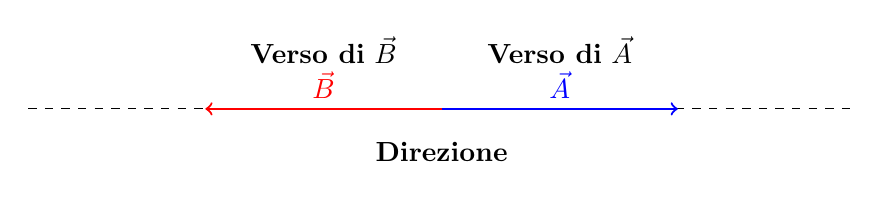
\begin{tikzpicture}[scale=1.5]
      % Disegno della direzione come linea tratteggiata
      \draw[dashed] (-3.5,0) -- (3.5,0);

      % Vettore A
      \draw[->, thick, blue] (0,0) -- (2,0) node[midway, above] {$\vec{A}$};

      % Vettore B
      \draw[<-, thick, red] (-2,0) -- (0,0) node[midway, above] {$\vec{B}$};

      % Etichette per la direzione e verso
      \node[above] at (1, 0.3) {\textbf{Verso di} $\vec{A}$};
      \node[above] at (-1, 0.3) {\textbf{Verso di} $\vec{B}$};
      \node[below] at (0, -0.2) {\textbf{Direzione}};
    \end{tikzpicture}
  \end{center}
  \leavevmode\\
  In questo esempio:
  \begin{itemize}
    \item \textbf{Direzione:} Entrambi i vettori \(\vec{A}\) e
      \(\vec{B}\) giacciono sulla stessa retta (la linea
      tratteggiata) e hanno la stessa direzione.
    \item \textbf{Verso:} Il vettore \(\vec{A}\) punta verso destra,
      mentre il vettore \(\vec{B}\) punta verso sinistra, quindi i
      due vettori hanno versi opposti.
  \end{itemize}
\end{nota}
\leavevmode\\\\
$AB=\{\text{Tutti i segmenti orientati, equipollenti ad }AB\}=\text{Vettore geometrico}$
\leavevmode\\\\
$\overrightarrow{AB}=\overrightarrow{CD}\Leftrightarrow AB\sim CD$
\leavevmode\\\\
$\overrightarrow{AB}+\overrightarrow{CD}=\overrightarrow{AB}+\overrightarrow{BE}=\overrightarrow{AE}\sim\text{Vettore geometrico rappresentato dal segmento orientato AE}$

\section{La somma Vettoriale è un gruppo Abeliano}

$\overrightarrow{AB}+\overrightarrow{BB}=\overrightarrow{AB}$

\begin{nota}
  $\overrightarrow{BB}$ Vettore geometrico nullo
\end{nota}
\leavevmode\\
$\overrightarrow{AB}+\overrightarrow{BA}=\overrightarrow{AA}$
\leavevmode\\
\begin{nota}
  $\overrightarrow{BA}$ Vettore geometrico opposto
\end{nota}
\leavevmode\\
\begin{wrapfigure}{r}{7cm}
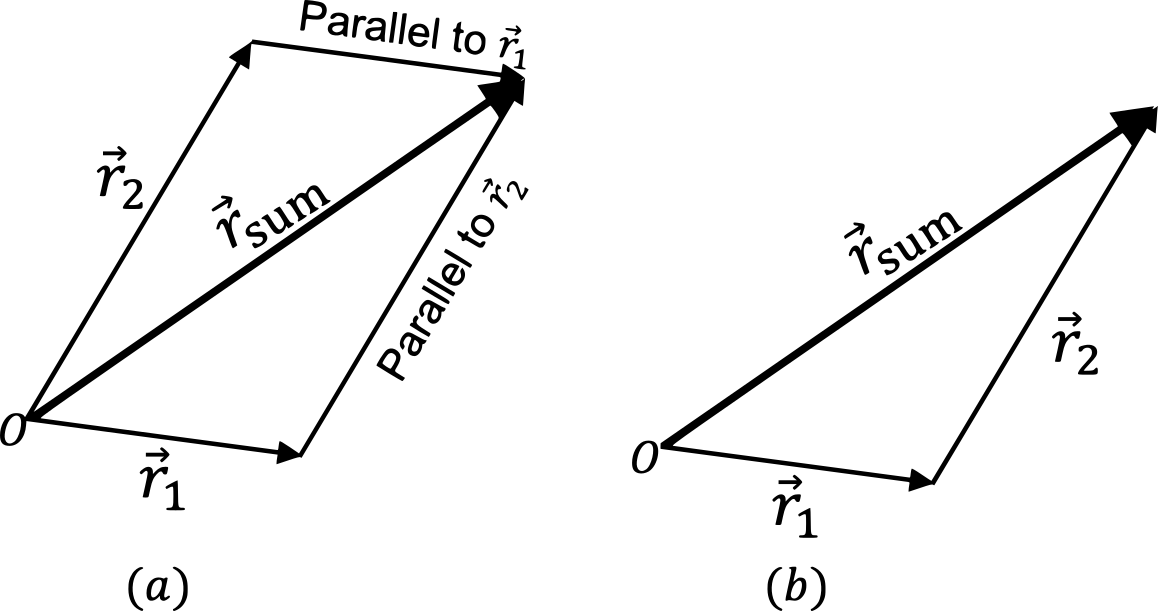
\includegraphics[height=0.28\textwidth]{Figures/somma tra vettori.pdf}
\end{wrapfigure} 

$\overrightarrow{U}+\overrightarrow{V}=\overrightarrow{V}+\overrightarrow{U}$
\leavevmode\\
\begin{flalign*}
  \overrightarrow{U}=\overrightarrow{AB}   & &\overrightarrow{U}+\overrightarrow{V}=\overrightarrow{AC}
  &&&&&&&&&&&&&&&&&&&&&&&&&&&&&&&&&&\\
  \overrightarrow{V}=\overrightarrow{BC}   &
  \phantom{...}\overrightarrow{V}=\overrightarrow{AD}\Rightarrow
  &\overrightarrow{U}=\overrightarrow{DC}  &&&&&&&&&&&&&&&&&&&&&&&&&&&&&&&&&&\\
  &
  &\overrightarrow{V}+\overrightarrow{U}=\overrightarrow{AC}
  &&&&&&&&&&&&&&&&&&&&&&&&&&&&&&&&&&
\end{flalign*}
\leavevmode\\\\\\\\\\\\
$(\overrightarrow{U}+\overrightarrow{V})+\overrightarrow{W}=\overrightarrow{U}+(\overrightarrow{V}+\overrightarrow{W})$
\leavevmode\\
\begin{flalign*}
	\overrightarrow{U}+\overrightarrow{V}		&=\overrightarrow{AC}	& &&&&&&&&&&&&&&&&&&&&&&&&&&&&&&&&&&&&&&&&&&&&&&&&&&&&&&&&&&&&&&&&&&&&&&&&&&&& \\
	(\overrightarrow{U}+\overrightarrow{W})+\overrightarrow{W}	&=\overrightarrow{AC}+\overrightarrow{CD}	&=\overrightarrow{AD} &&&&&&&&&&&&&&&&&&&&&&&&&&&&&&&&&&&&&&&&&&&&&&&&&&&&&&&&&&&&&&&&&&&&&&&&&&&&
\end{flalign*}

\leavevmode\\
\begin{flalign*}
	\overrightarrow{V}+\overrightarrow{W}		&=\overrightarrow{BD}	& &&&&&&&&&&&&&&&&&&&&&&&&&&&&&&&&&&&&&&&&&&&&&&&&&&&&&&&&&&&&&&&&&&&&&&&&&&&& \\
	\overrightarrow{U}+(\overrightarrow{W}+\overrightarrow{W})	&=\overrightarrow{AB}+\overrightarrow{BD}	&=\overrightarrow{AD} &&&&&&&&&&&&&&&&&&&&&&&&&&&&&&&&&&&&&&&&&&&&&&&&&&&&&&&&&&&&&&&&&&&&&&&&&&&&
\end{flalign*}

\begin{align*}
	\beta\cdot \overrightarrow{u}
	\begin{cases}
		\text{Se } \beta=0 \text{ o } \overrightarrow{u}=0 \Rightarrow& \overrightarrow{0}\\
		\text{Se } \beta\neq0 \text{ e } \overrightarrow{u}\neq 0 \Rightarrow& \text{Stessa direzione di }\overrightarrow{u}\\
		\text{Se e solo se } \beta\neq0 \Rightarrow& \text{Stesso verso di } \overrightarrow{u}
	\end{cases}\\
	\beta\in\mathbb{R}
\end{align*}

$$|\beta\cdot\overrightarrow{u}|=|\beta|\cdot|\overrightarrow{u}|$$

\begin{esercizio}
	Addizione di Vettori
	\leavevmode\\
	Siano dati i vettori 
	\[
	\vec{u} = \begin{bmatrix} 2 \\ 3 \end{bmatrix} \quad \text{e} \quad \vec{v} = \begin{bmatrix} 4 \\ 1 \end{bmatrix}.
	\]
	Calcola \(\vec{u} + \vec{v}\).
	\leavevmode\\
	\[
	\vec{u} + \vec{v} = \begin{bmatrix} 2 \\ 3 \end{bmatrix} + \begin{bmatrix} 4 \\ 1 \end{bmatrix} = \begin{bmatrix} 6 \\ 4 \end{bmatrix}
	\]
	\leavevmode\\
	\textbf{Rappresentazione Grafica:}
	\leavevmode\\
	\begin{center}
		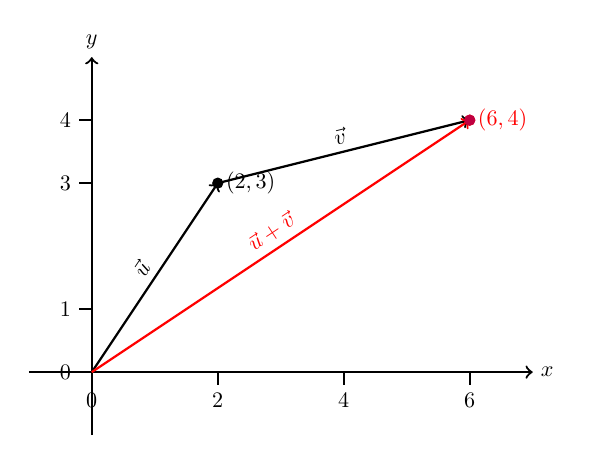
\begin{tikzpicture}[thick,scale=0.8, every node/.style={scale=0.8}]
			% Assi con tacche
			\draw[->] (-1,0) -- (7,0) node[right] {$x$};
			\foreach \x in {0, 2, 4, 6} \draw (\x,0) -- (\x,-0.2) node[below] {\x};
			\draw[->] (0,-1) -- (0,5) node[above] {$y$};
			\foreach \y in {0, 1, 3, 4} \draw (0,\y) -- (-0.2,\y) node[left] {\y};
			
			% Vettore u
			\draw[->, thick, black] (0,0) -- (2,3) node[midway, above, sloped] {$\vec{u}$};
			\filldraw[black] (2,3) circle (2pt) node[right] {$(2, 3)$};
			
			% Vettore v
			\draw[->, thick, black] (2,3) -- (6,4) node[midway, above, sloped] {$\vec{v}$};
			\filldraw[red] (6,4) circle (2pt) node[right] {$(6, 4)$};
			
			% Vettore risultante u + v
			\draw[->, thick, red] (0,0) -- (6,4) node[midway, above, sloped] {$\vec{u} + \vec{v}$};
			\filldraw[purple] (6,4) circle (2pt);
		\end{tikzpicture}
	\end{center}
\end{esercizio}
\newpage
\begin{esercizio}
	Sottrazione di Vettori
	\leavevmode\\
	Siano dati i vettori 
	\[
	\vec{u} = \begin{bmatrix} 5 \\ 2 \end{bmatrix} \quad \text{e} \quad \vec{v} = \begin{bmatrix} 2 \\ 3 \end{bmatrix}.
	\]
	Calcola \(\vec{u} - \vec{v}\).
	\leavevmode\\
	\[
	\vec{u} - \vec{v} = \begin{bmatrix} 5 \\ 2 \end{bmatrix} - \begin{bmatrix} 2 \\ 3 \end{bmatrix} = \begin{bmatrix} 3 \\ -1 \end{bmatrix}
	\]
	\leavevmode\\
	\textbf{Rappresentazione Grafica:}
	\leavevmode\\
	\begin{center}
		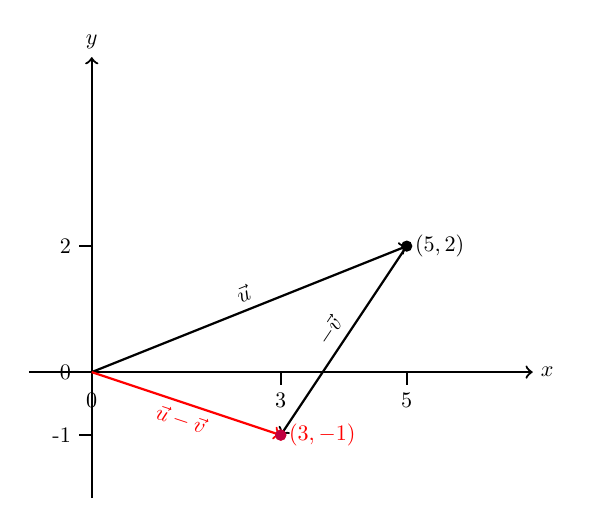
\begin{tikzpicture}[thick,scale=0.8, every node/.style={scale=0.8}]
			% Assi con tacche
			\draw[->] (-1,0) -- (7,0) node[right] {$x$};
			\foreach \x in {0, 3, 5} \draw (\x,0) -- (\x,-0.2) node[below] {\x};
			\draw[->] (0,-2) -- (0,5) node[above] {$y$};
			\foreach \y in {-1, 0, 2} \draw (0,\y) -- (-0.2,\y) node[left] {\y};
			
			% Vettore u
			\draw[->, thick, black] (0,0) -- (5,2) node[midway, above, sloped] {$\vec{u}$};
			\filldraw[black] (5,2) circle (2pt) node[right] {$(5, 2)$};
			
			% Vettore -v
			\draw[->, thick, black] (5,2) -- (3,-1) node[midway, above, sloped] {$-\vec{v}$};
			\filldraw[red] (3,-1) circle (2pt) node[right] {$(3, -1)$};
			
			% Vettore risultante u - v
			\draw[->, thick, red] (0,0) -- (3,-1) node[midway, below, sloped] {$\vec{u} - \vec{v}$};
			\filldraw[purple] (3,-1) circle (2pt);
		\end{tikzpicture}
	\end{center}
\end{esercizio}

\begin{esercizio}
	Moltiplicazione per uno Scalare
	\leavevmode\\
	Sia dato il vettore 
	\[
	\vec{u} = \begin{bmatrix} 1 \\ 4 \end{bmatrix}.
	\]
	Calcola \(2 \vec{u}\).
	\leavevmode\\
	\[
	\frac{1}{2} \vec{u} = \frac{1}{2} \cdot \begin{bmatrix} 1 \\ 4 \end{bmatrix} = \begin{bmatrix} 0,5 \\ 2 \end{bmatrix}
	\]
	\leavevmode\\
	\textbf{Rappresentazione Grafica:}
	\leavevmode\\
	\begin{center}
		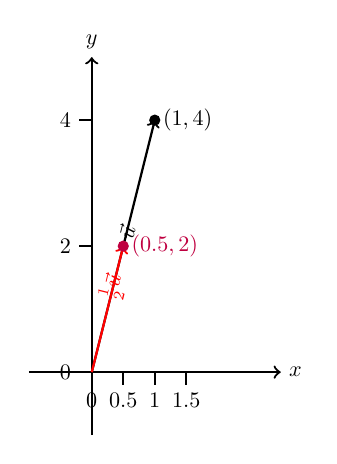
\begin{tikzpicture}[thick,scale=0.8, every node/.style={scale=0.8}]
			% Assi con tacche
			\draw[->] (-1,0) -- (3,0) node[right] {$x$};
			\foreach \x in {0, 0.5, 1, 1.5} \draw (\x,0) -- (\x,-0.2) node[below] {\x};
			\draw[->] (0,-1) -- (0,5) node[above] {$y$};
			\foreach \y in {0, 2, 4} \draw (0,\y) -- (-0.2,\y) node[left] {\y};
			
			% Vettore u
			\draw[->, thick, black] (0,0) -- (1,4) node[midway, right, sloped] {$\vec{u}$};
			\filldraw[black] (1,4) circle (2pt) node[right] {$(1, 4)$};
			
			% Vettore risultante 1/2 u
			\draw[->, thick, red] (0,0) -- (0.5,2) node[midway, right, sloped] {$\frac{1}{2}\vec{u}$};
			\filldraw[purple] (0.5,2) circle (2pt) node[right] {$(0.5, 2)$};
		\end{tikzpicture}
	\end{center}
\end{esercizio}

\section{Prodotto scalare standard in $\mathbb{R}^n$}

\begin{flalign*}
	\begin{cases}
		\underline{a}=(a_1,\dots,a_n) \\
		\underline{b}=(b_1,\dots,b_n)
	\end{cases}
	,\underline{a}\cdot\underline{b}=a_1\cdot b_1+a_2\cdot b_2+\dots+a_n\cdot b_n=\sum_{i=1}^{n} a_i\cdot b_i
\end{flalign*}

\begin{nota}
	Il risultato è uno scalare e non un vettore
\end{nota}

$$\underline{a}\cdot \underline{b}=\underline{b}\cdot \underline{a}, \phantom{text} \underline{a}\cdot \underline{0}=0, \phantom{text} \underline{a}\cdot(\underline{b}+\underline{c})=\underline{a}\cdot \underline{b}+\underline{a}\cdot \underline{c}$$

\begin{nota}
	$\underline{a}\cdot\underline{b}$ può essere $0$ anche se $\underline{a}$ e $\underline{b}$ sono diversi da $\underline{0}$
\end{nota}

\begin{es}
	\begin{flalign*}
		(1,3,1)\cdot(1,-2,-3)&=&1-6-3&=&-8&&&&&&&&&&&&&&&&&&&&&&\\
		(1,2,3)\cdot(3,0,-1)&=&3+0-3&=&0&&&&&&&&&&&&&&&&&&&&&&\\
		(1,1,1)\cdot(1,0,-1)&=&1+0-1&=&0&&&&&&&&&&&&&&&&&&&&&&
	\end{flalign*}
\end{es}

\section{Prodotto righe per colonne}

Quando si parla di prodotto righe per colonne, si fa riferimento al prodotto scalare tra una riga di una matrice e una colonna di un’altra matrice. Questa operazione risulta particolarmente utile nel calcolo del prodotto tra matrici, in cui ciascun elemento della matrice risultante si ottiene moltiplicando ogni elemento della riga di una matrice per il corrispondente elemento della colonna dell’altra e sommando poi i prodotti ottenuti.

Formalmente, se abbiamo una matrice \( A \) di dimensioni \( m \times n \) e una matrice \( B \) di dimensioni \( n \times p \), il prodotto di \( A \) e \( B \) (denotato come \( A \cdot B \)) è una matrice \( C \) di dimensioni \( m \times p \), in cui ciascun elemento \( c_{ij} \) è calcolato come:

\[
c_{ij} = \sum_{k=1}^n a_{ik} \cdot b_{kj}
\]

In altre parole, l'elemento nella posizione \( (i, j) \) della matrice \( C \) è il risultato del prodotto scalare tra la \( i \)-esima riga di \( A \) e la \( j \)-esima colonna di \( B \). Questo tipo di prodotto è fondamentale anche nel caso di vettori riga e vettori colonna, poiché permette di ottenere scalari, vettori o matrici a seconda della disposizione iniziale dei vettori coinvolti.

\begin{nota}
	Attenzione\\
	$A_{m\times \highlight{n}} \cdot B_{\highlight{n}\times p}$\\
	Il numero di colonne della prima matrice deve essere uguale al numero di colonne della seconda matrice!
\end{nota}













